\documentclass{beamer}
\usepackage[utf8]{inputenc}

\usetheme{Madrid}
\usecolortheme{default}
\useinnertheme{circles}

\definecolor{Logo1}{rgb}{0.208, 0.2865, 0.373}
\definecolor{Logo2}{rgb}{0.000, 0.674, 0.863}

\setbeamercolor*{palette primary}{bg=Logo1, fg=white}
\setbeamercolor*{palette secondary}{bg=Logo2, fg=white}
\setbeamercolor*{palette tertiary}{bg=white, fg=Logo1}
\setbeamercolor*{palette quaternary}{bg=Logo1,fg=white}
\setbeamercolor{structure}{fg=Logo1} % itemize, enumerate, etc
\setbeamercolor{section in toc}{fg=Logo1} % TOC sections

\usepackage{graphicx,animate}
%------------------------------------------------------------
%This block of code defines the information to appear in the
%Title page
\title[Linear Algebra] %optional
{Gram-Schmidt; Introduction to Determinant}

\subtitle{Lecture 8}

\author[11910803@mail.sustech.edu.cn] % (optional)
{
    Zhang Ce
}

\institute[] % (optional)
{
    Department of Electrical and Electronic Engineering\\
    Southern University of Science and Technology
}

\date[2021.11.16] % (optional)
{2021.11.16}


%End of title page configuration block
%------------------------------------------------------------



%------------------------------------------------------------
%The next block of commands puts the table of contents at the
%beginning of each section and highlights the current section:

\AtBeginSection[]
{
\begin{frame}
    \frametitle{Table of Contents}
    \tableofcontents[currentsection]
\end{frame}
}
%------------------------------------------------------------


\begin{document}

%The next statement creates the title page.
\frame{\titlepage}


%---------------------------------------------------------
%This block of code is for the table of contents after
%the title page
\begin{frame}
\frametitle{Table of Contents}
\tableofcontents
\end{frame}
%---------------------------------------------------------
\section{A Brief Review of Last Lecture}
\begin{frame}{Last Lecture, We Discuss\dots}
Four parts in last lecture:
    \begin{enumerate}
        \item Orthogonal Vector and Subspaces\\
        inner product (dot product), definition of orthogonality
        \item Projection onto Lines\\
        geometrical interpretation, projection matrix
        \item Least Squares\\
        geometrical view and general projection matrices
        \item Interesting Applications of Linear Algebra\\
        chemistry, circuit principles and computer vision
    \end{enumerate}

\end{frame}

\begin{frame}{Least-Squares}
The core is: find the solution for $Ax=p$ (A is the matrix with $a_1,a_2$ in columns) where $p$ is the projection on $C(A)$, which can definitely gives a unique solution.

\begin{figure}
    \centering
    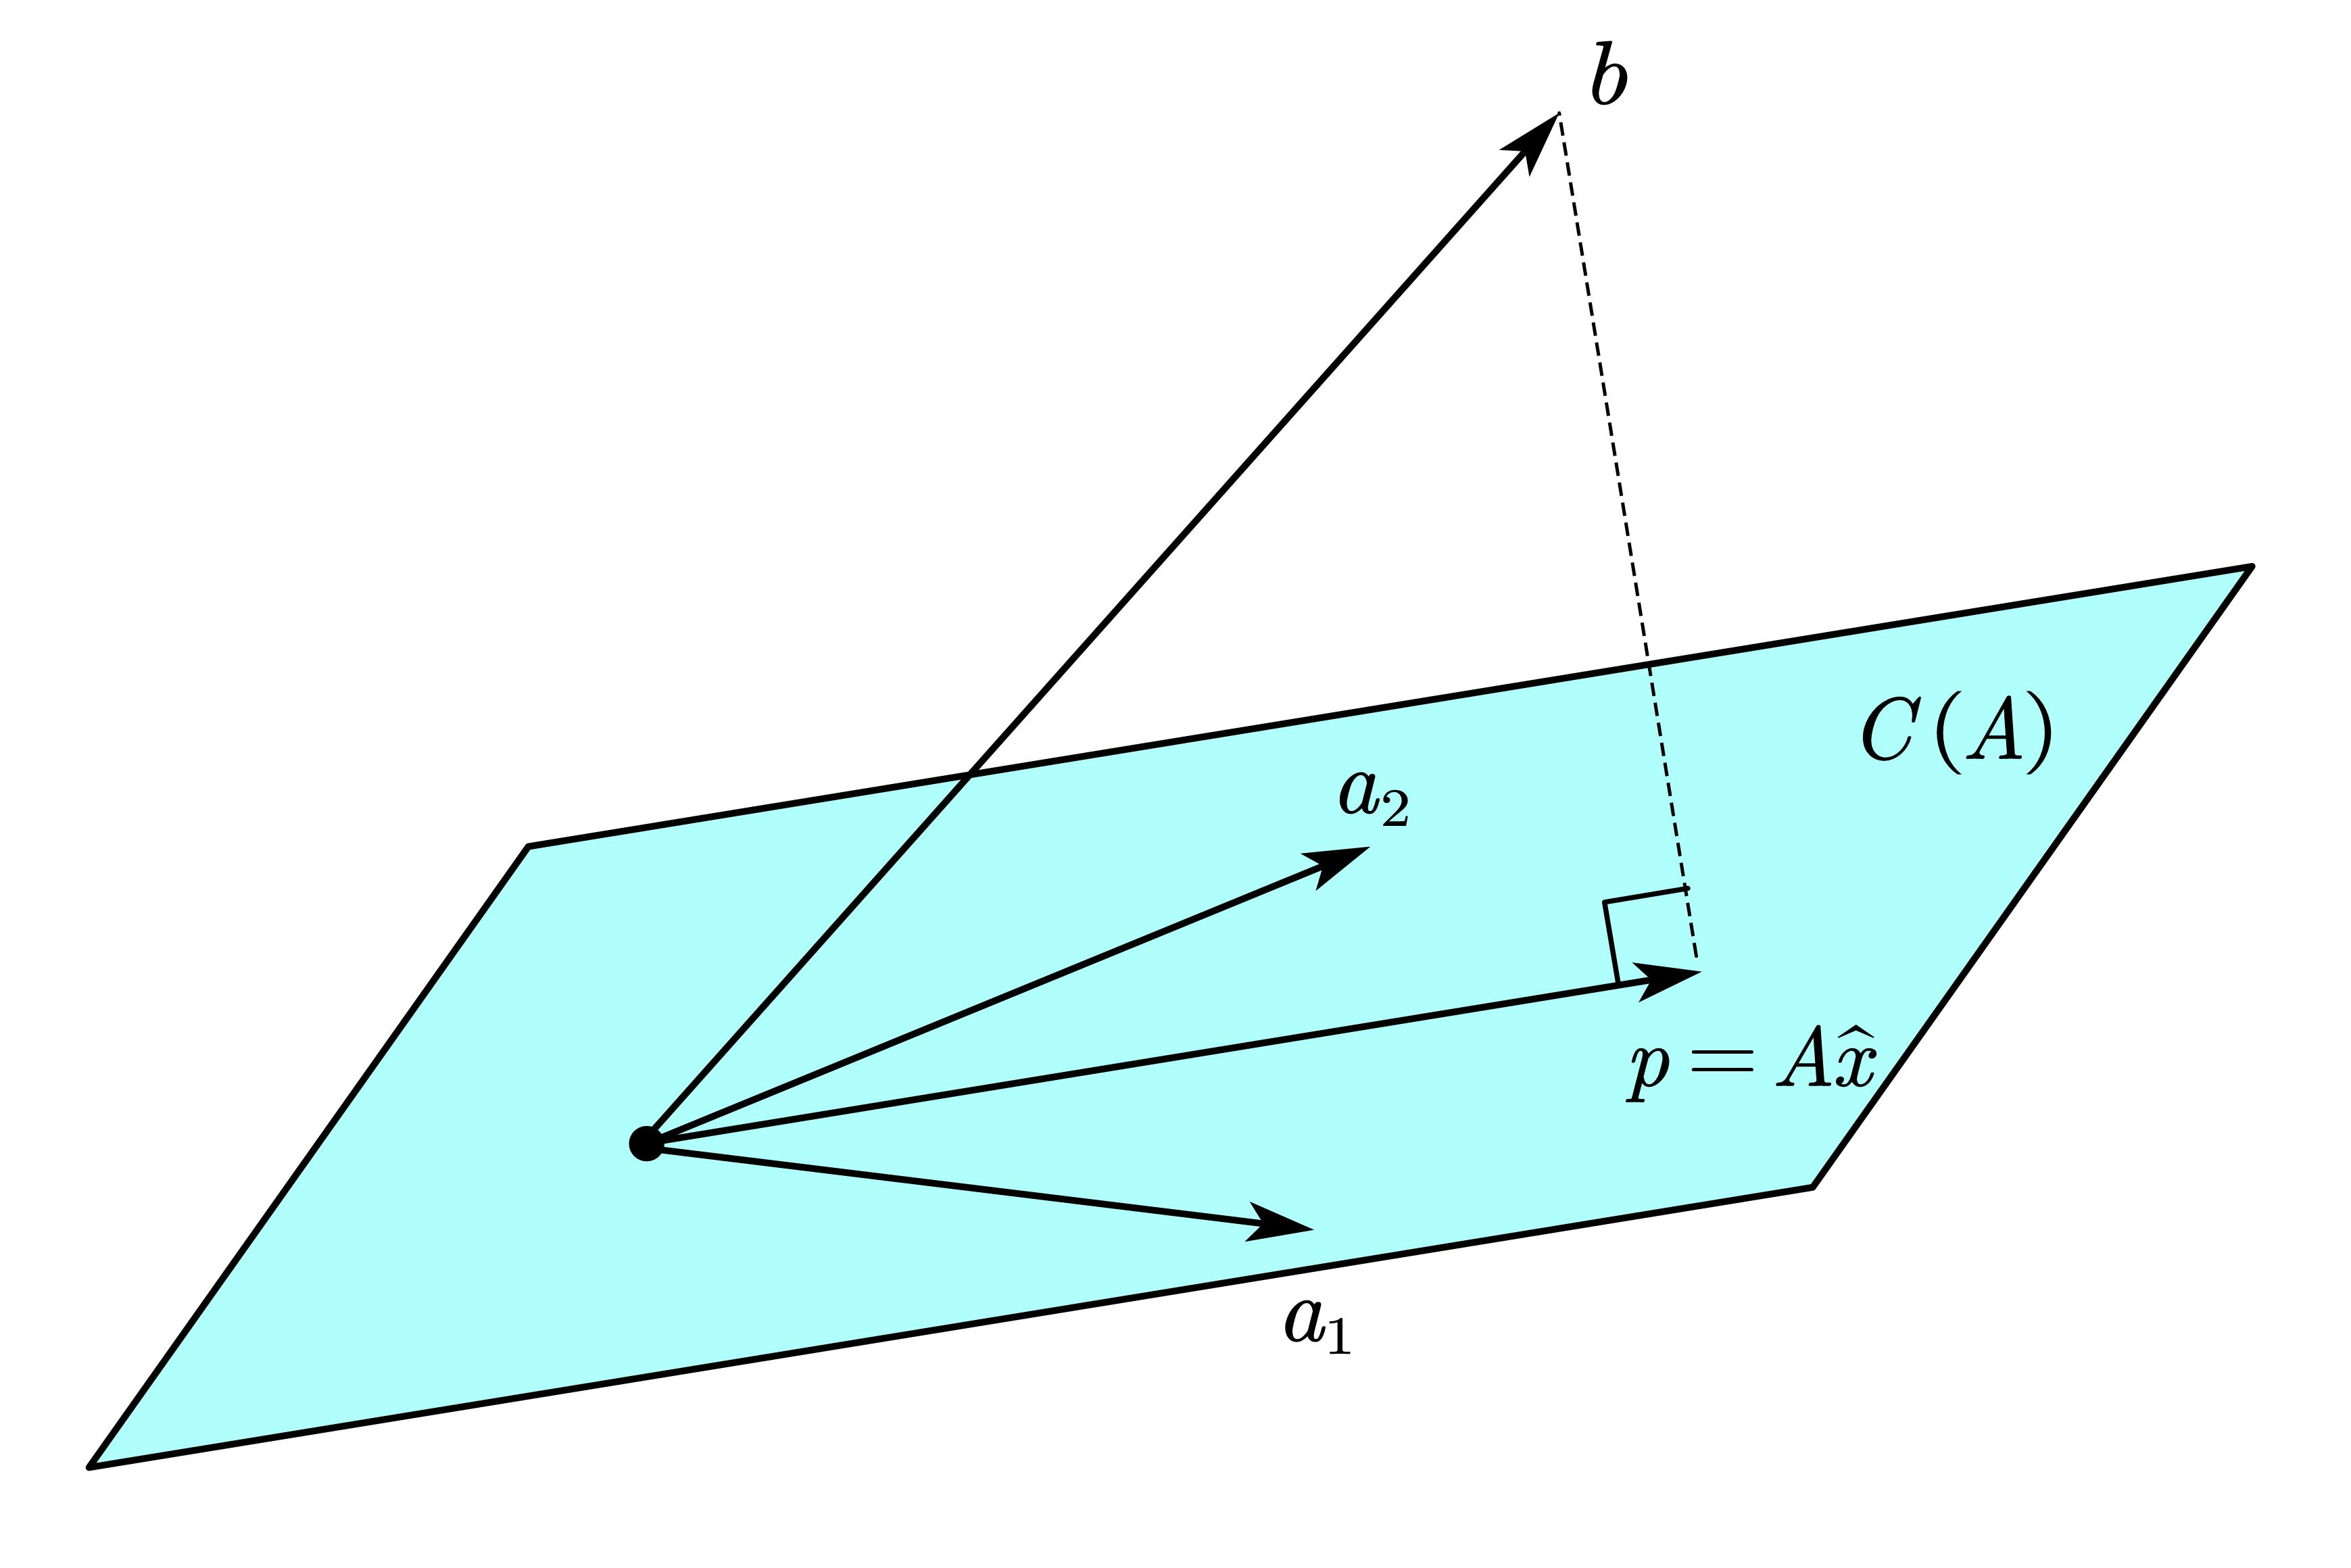
\includegraphics[width=0.5\textwidth]{ls.jpg}
\end{figure}
\begin{equation*}
    {a_1}^T\left( b-A\hat{x} \right) ={a_2}^T\left( b-A\hat{x} \right) =0
\end{equation*}

The error $e=b-p=b-A\hat{x}$ is in the nullspace of $A$, while the projection $p=A\hat{x}$ is in the column space of $A$!
\end{frame}

\begin{frame}{Least-Squares}
We can simplify that equation...
    \begin{equation*}
        {a_1}^T\left( b-A\hat{x} \right) ={a_2}^T\left( b-A\hat{x} \right) =0
    \end{equation*}
\begin{equation*}
    \left[ \begin{array}{c}
        {a_1}^T\\
        {a_2}^T\\
    \end{array} \right] \left( b-A\hat{x} \right) =\left[ \begin{array}{c}
        0\\
        0\\
    \end{array} \right]
\end{equation*}
\begin{equation*}
    A^T\left( b-A\hat{x} \right) =0
\end{equation*}
\begin{equation*}
    A^TA\hat{x} =A^Tb
\end{equation*}

Now, can you tell me why $A^TA\hat{x} =A^Tb$ must be consistent? The reason behind: $Ax=p$ must have solutions.

\vspace{3pt}
Finally, we can get:
\begin{equation*}
    \hat{x} =(A^TA)^{-1}A^Tb
\end{equation*}

That is the least-squares solution, indicating how to combine the columns in $A$ can we get the nearest vector to $b$.
\end{frame}

\begin{frame}{Projection Matrices}
The projection vector in the column space, which is also the nearest vector to $b$ in $C(A)$:
\begin{equation*}
    p=A\hat{x}=A\left( A^TA \right) ^{-1}A^Tb=Pb
\end{equation*}

Now we can have projection matrices onto column space of $A$:
\begin{equation*}
    P=A\left( A^TA \right) ^{-1}A^T
\end{equation*}

Can I take the inverse and simplify the expression further?
\begin{equation*}
    P=A\left( A^TA \right) ^{-1}A^T=AA^{-1}(A^T)^{-1}A^T=I\:???
\end{equation*}

$A$ is not square matrix, $A^{-1}$ doesn't exist.

\vspace{3pt}
Recall that we have introduced projection matrices onto lines:
\begin{equation*}
    P=\frac{\mathbf{aa}^T}{\mathbf{a}^T\mathbf{a}}
\end{equation*}

It is just a special case (1-D case) for projection matrices.
\end{frame}

\begin{frame}{Linear Algebra in Chemistry}
Balance the chemical reaction equation:
\begin{equation*}
    P_4+CuSO_4+H_2O\rightarrow Cu_3P+H_2SO_4+H_3PO_4
\end{equation*}

\begin{itemize}
    \item For element $P$: $4x_1=x_4+x_6$.
    \item For element $Cu$: $x_2=3x_4$.
    \item For element $S$: $x_2=x_5$.
    \item For element $O$: $4x_2+x_3=4x_5+4x_6$.
    \item For element $H$: $2x_3=2x_5+3x_6$.
\end{itemize}

\begin{equation*}
    \left[ \begin{matrix}
        4&		0&		0&		-1&		0&		-1\\
        0&		1&		0&		-3&		0&		0\\
        0&		1&		0&		0&		-1&		0\\
        0&		4&		1&		0&		-4&		-4\\
        0&		0&		2&		0&		-2&		-3\\
    \end{matrix} \right]
\end{equation*}

Guess the rank of the matrix, give explanations also.
\end{frame}

\begin{frame}{Linear Algebra in Chemistry}
\begin{equation*}
    \left[ \begin{matrix}
        4&		0&		0&		-1&		0&		-1\\
        0&		1&		0&		-3&		0&		0\\
        0&		1&		0&		0&		-1&		0\\
        0&		4&		1&		0&		-4&		-4\\
        0&		0&		2&		0&		-2&		-3\\
    \end{matrix} \right] \rightarrow \left[ \begin{matrix}
        4&		0&		0&		-1&		0&		-1\\
        0&		1&		0&		-3&		0&		0\\
        0&		0&		1&		12&		-4&		-4\\
        0&		0&		0&		3&		-1&		0\\
        0&		0&		0&		0&		-2&		5\\
    \end{matrix} \right]
\end{equation*}

Free variable $x_6$ set to 2, the solution is:
\begin{equation*}
    x=\left[ \begin{matrix}
        11/12&		5&		8&		5/3&		5&		2\\
    \end{matrix} \right] ^T
\end{equation*}

Multiply a constant 12, the solution becomes:
\begin{equation*}
    x=\left[ \begin{matrix}
        11&		60&		96&		20&		60&		24\\
    \end{matrix} \right] ^T
\end{equation*}

So, the final chemical reaction equation is:
\begin{equation*}
    11P_4+60CuSO_4+96H_2O= 20Cu_3P+60H_2SO_4+24H_3PO_4
\end{equation*}
\end{frame}

\begin{frame}{Linear Algebra in Circult Principles}
Can you figure out the whole state of the following circuit?

\begin{figure}
    \centering
    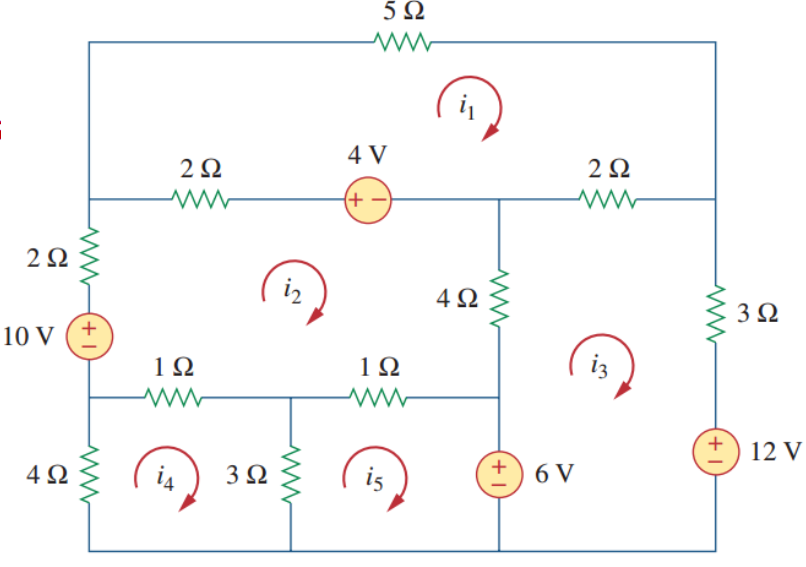
\includegraphics[width=0.6\textwidth]{example.png}
\end{figure}

Our method is: find the mesh current $i_1, i_2, i_3, i_4, i_5$.
\end{frame}

\begin{frame}{Linear Algebra in Circult Principles}
The essence: Solve $Ax=b$ linear system!
\begin{figure}
    \centering
    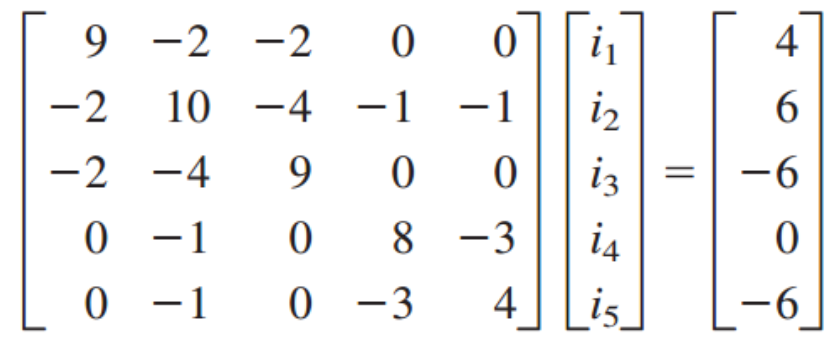
\includegraphics[width=0.6\textwidth]{eq.png}
\end{figure}

Every row is a KVL equation for a mesh.

\vspace{3pt}
If there is no voltage source, then the equation system becomes $Ax=0$, the mesh currents are definitely all zero (that is to say the matrix is of full rank because all the meshes are independent, no repeat meshes occur)!

\vspace{3pt}
The result will be
\begin{equation*}
    i_1=0.283A,i_2=0.211A,i_3=-0.488A,i_4=-0.718A,i_5=-1.986A
\end{equation*}

\end{frame}

\begin{frame}{Linear Algebra in Computer Vision}
A new operation: convolution.

\begin{figure}
    \centering
    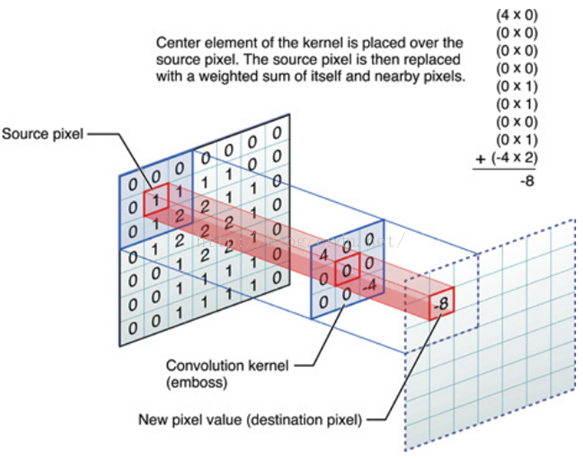
\includegraphics[width=0.6\textwidth]{conv.png}
\end{figure}

Now, let's see what will happen for different convolution kernel.
\end{frame}

\begin{frame}{Linear Algebra in Computer Vision}
    \begin{itemize}
        \item Identity Filter:
        \begin{figure}
            \centering
            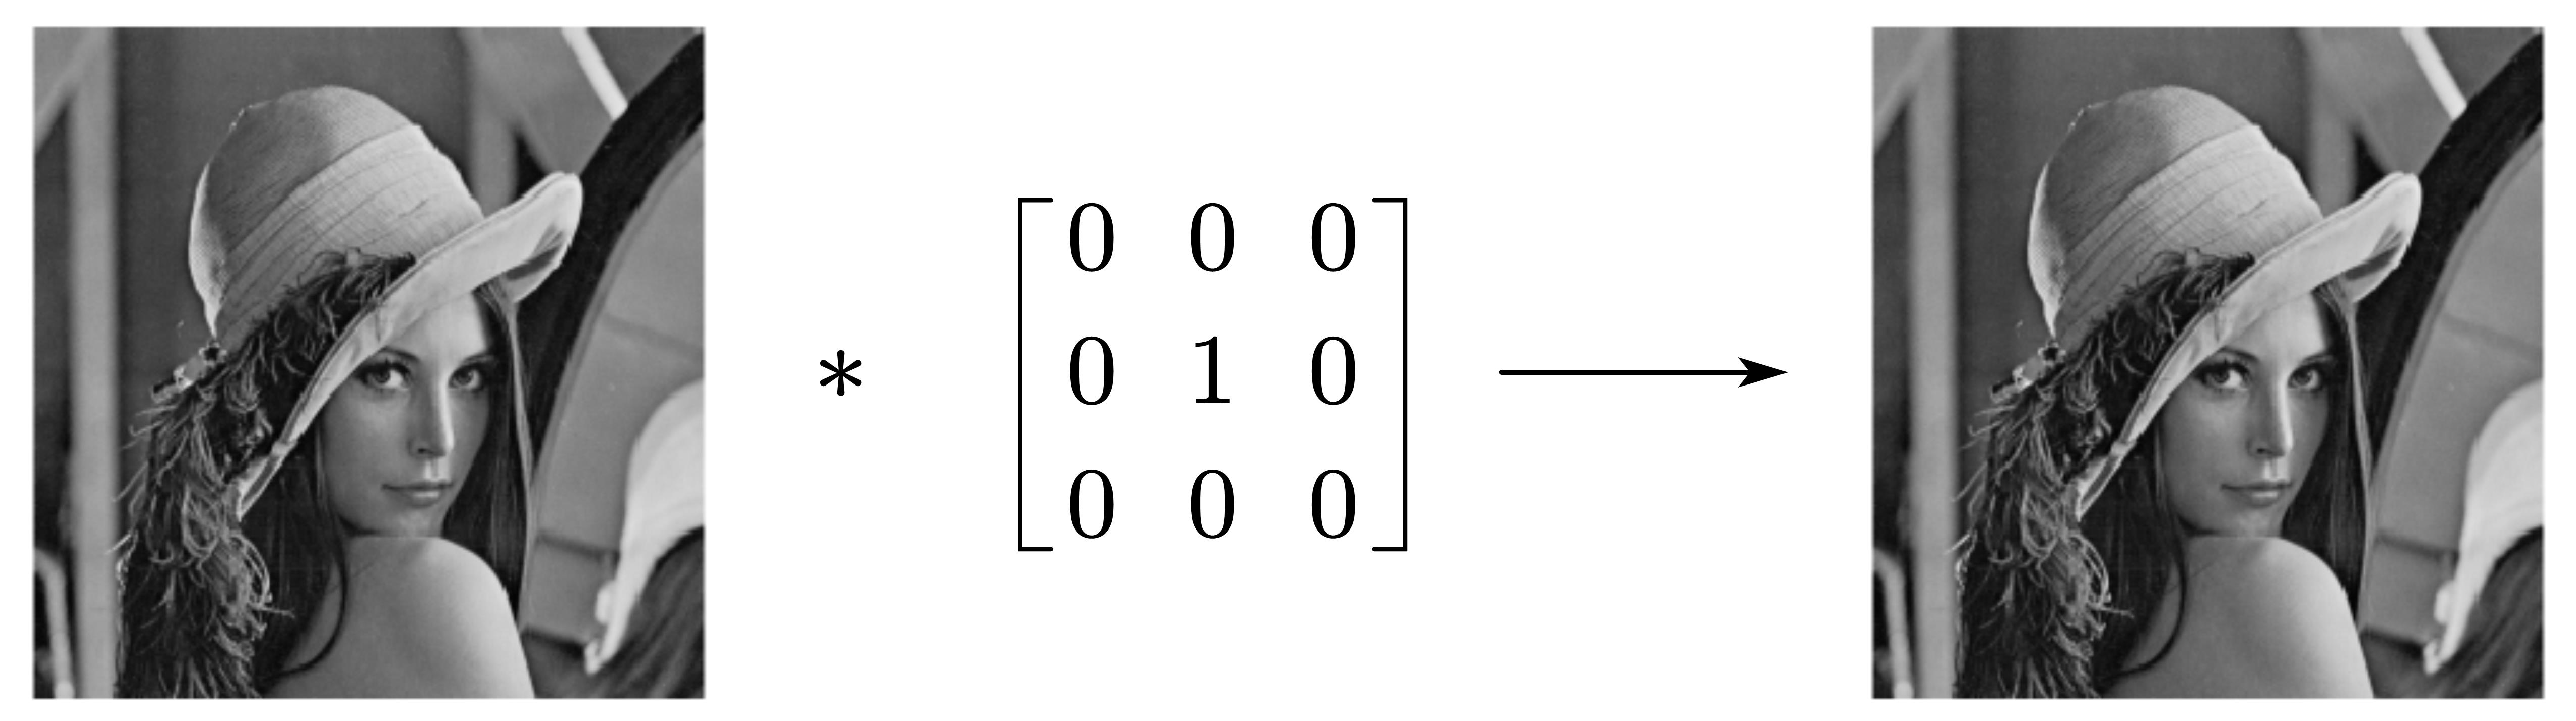
\includegraphics[width=0.8\textwidth]{lena1.jpg}
        \end{figure}
        \item Sharpness Filter (enhance contents):
        \begin{figure}
            \centering
            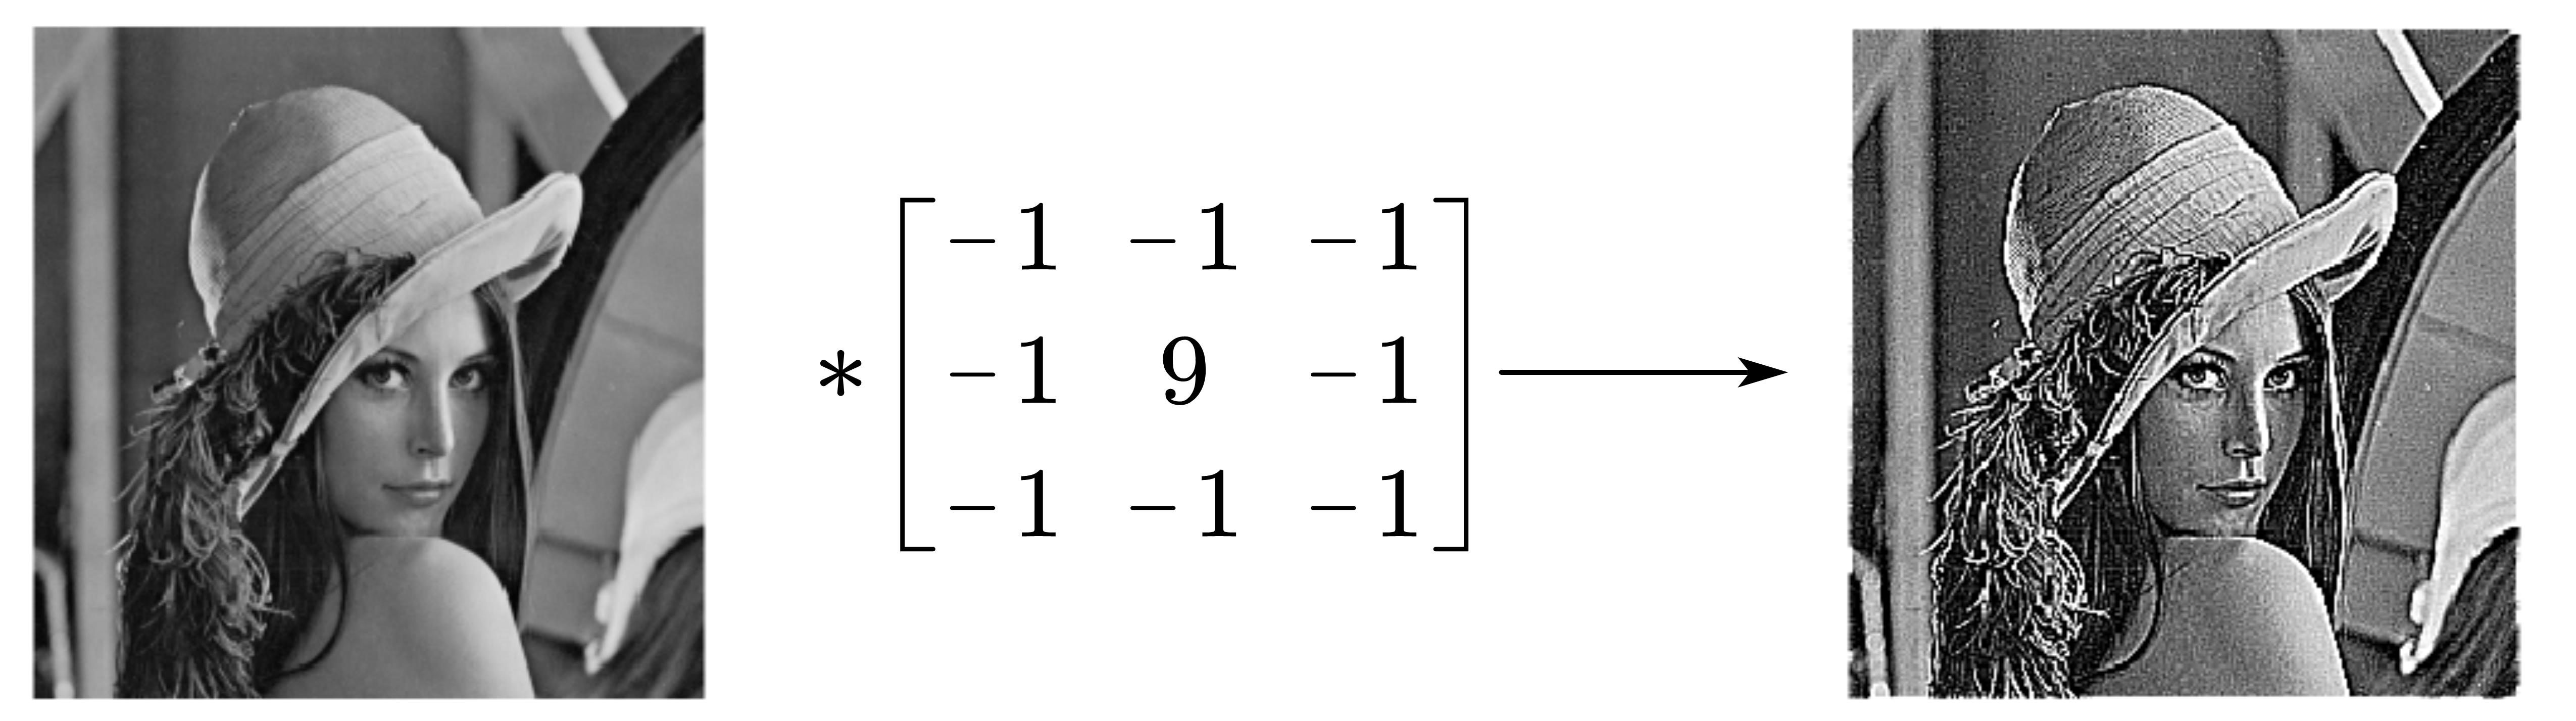
\includegraphics[width=0.8\textwidth]{lena2.jpg}
        \end{figure}
    \end{itemize}
\end{frame}

\begin{frame}{Linear Algebra in Computer Vision}
    \begin{itemize}
        \item Another Sharpness Filter (enhance edges):
        \begin{figure}
            \centering
            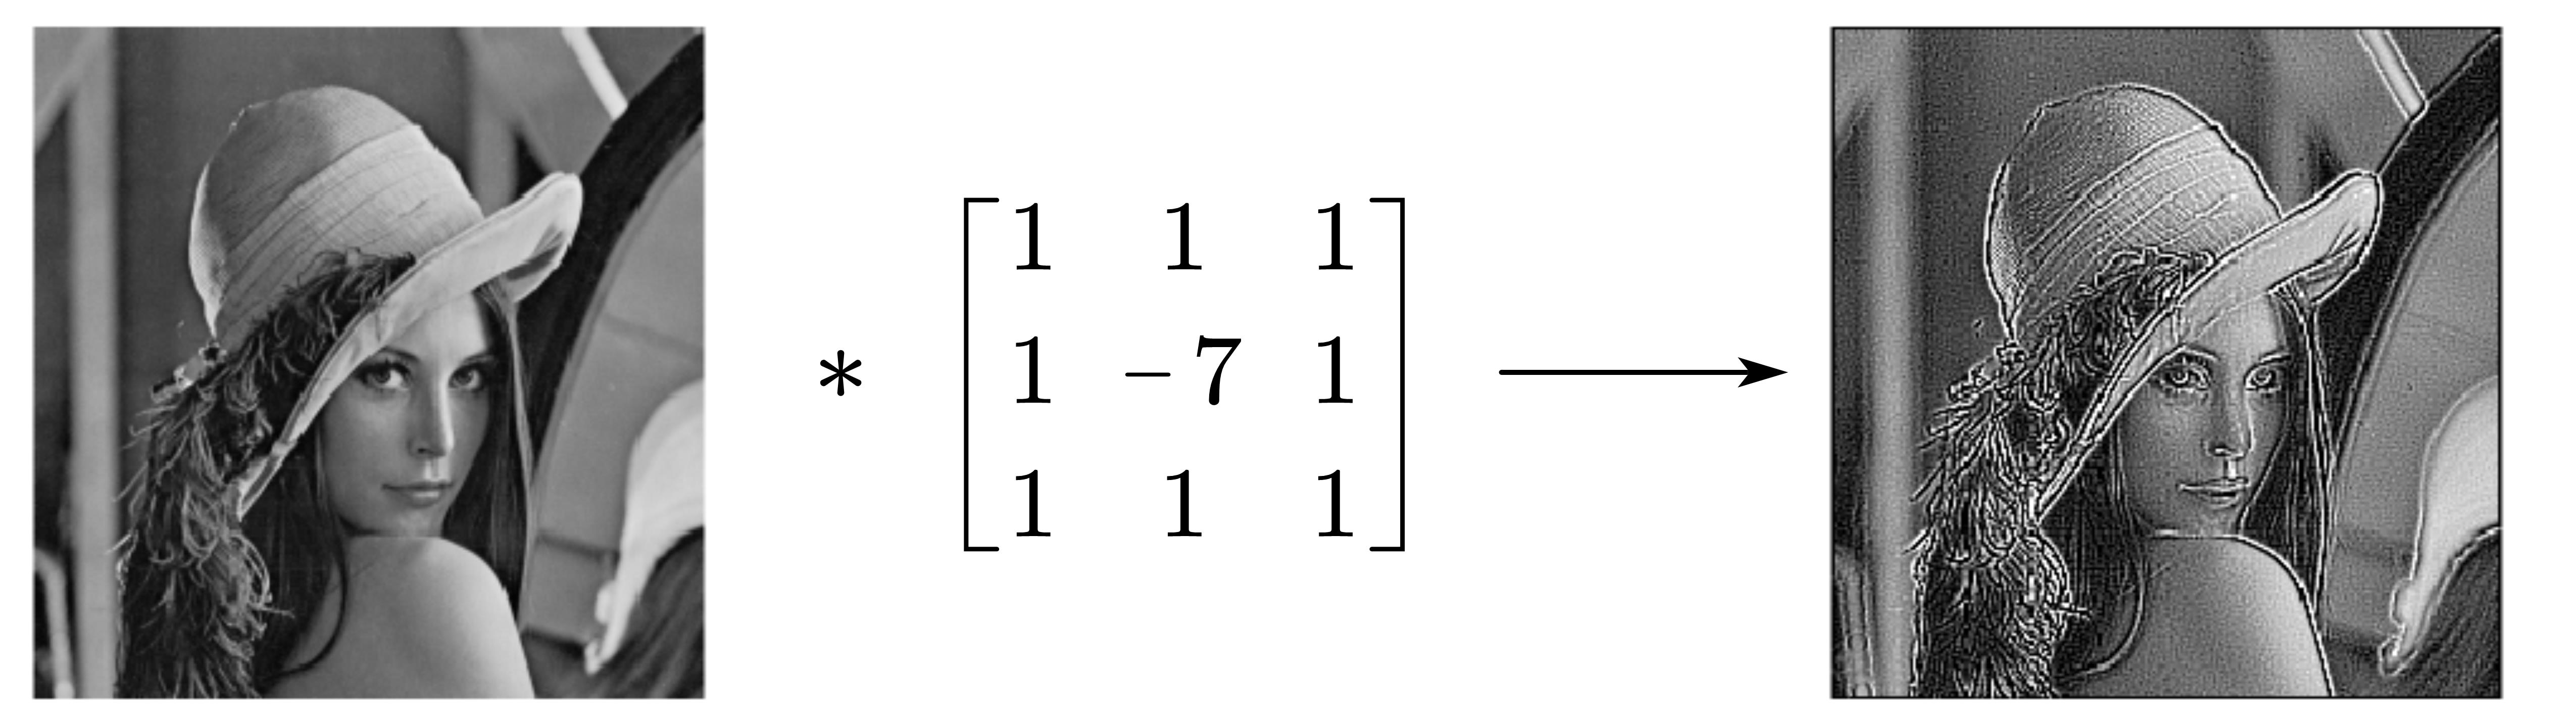
\includegraphics[width=0.8\textwidth]{lena3.jpg}
        \end{figure}
        \item Edge Detection Filter:
        \begin{figure}
            \centering
            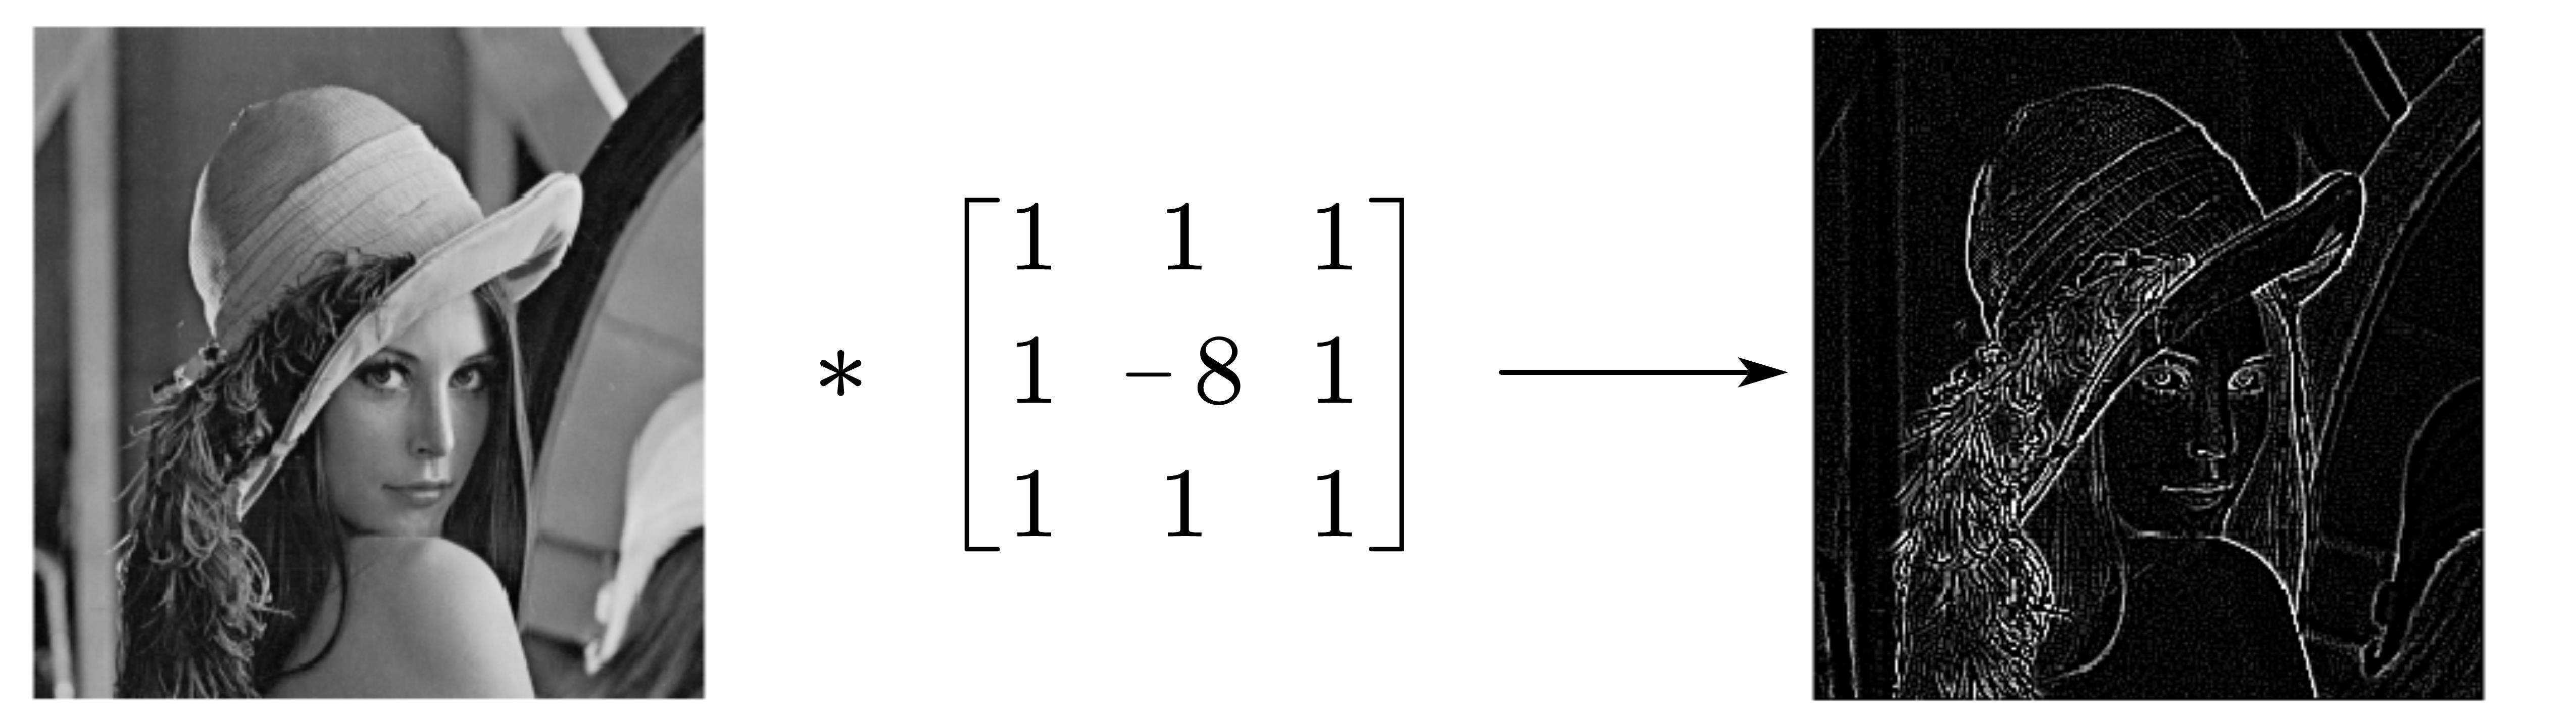
\includegraphics[width=0.8\textwidth]{lena4.jpg}
        \end{figure}
    \end{itemize}
\end{frame}

\begin{frame}{Linear Algebra in Computer Vision}
    \begin{itemize}
        \item Average Box Filter:
        \begin{figure}
            \centering
            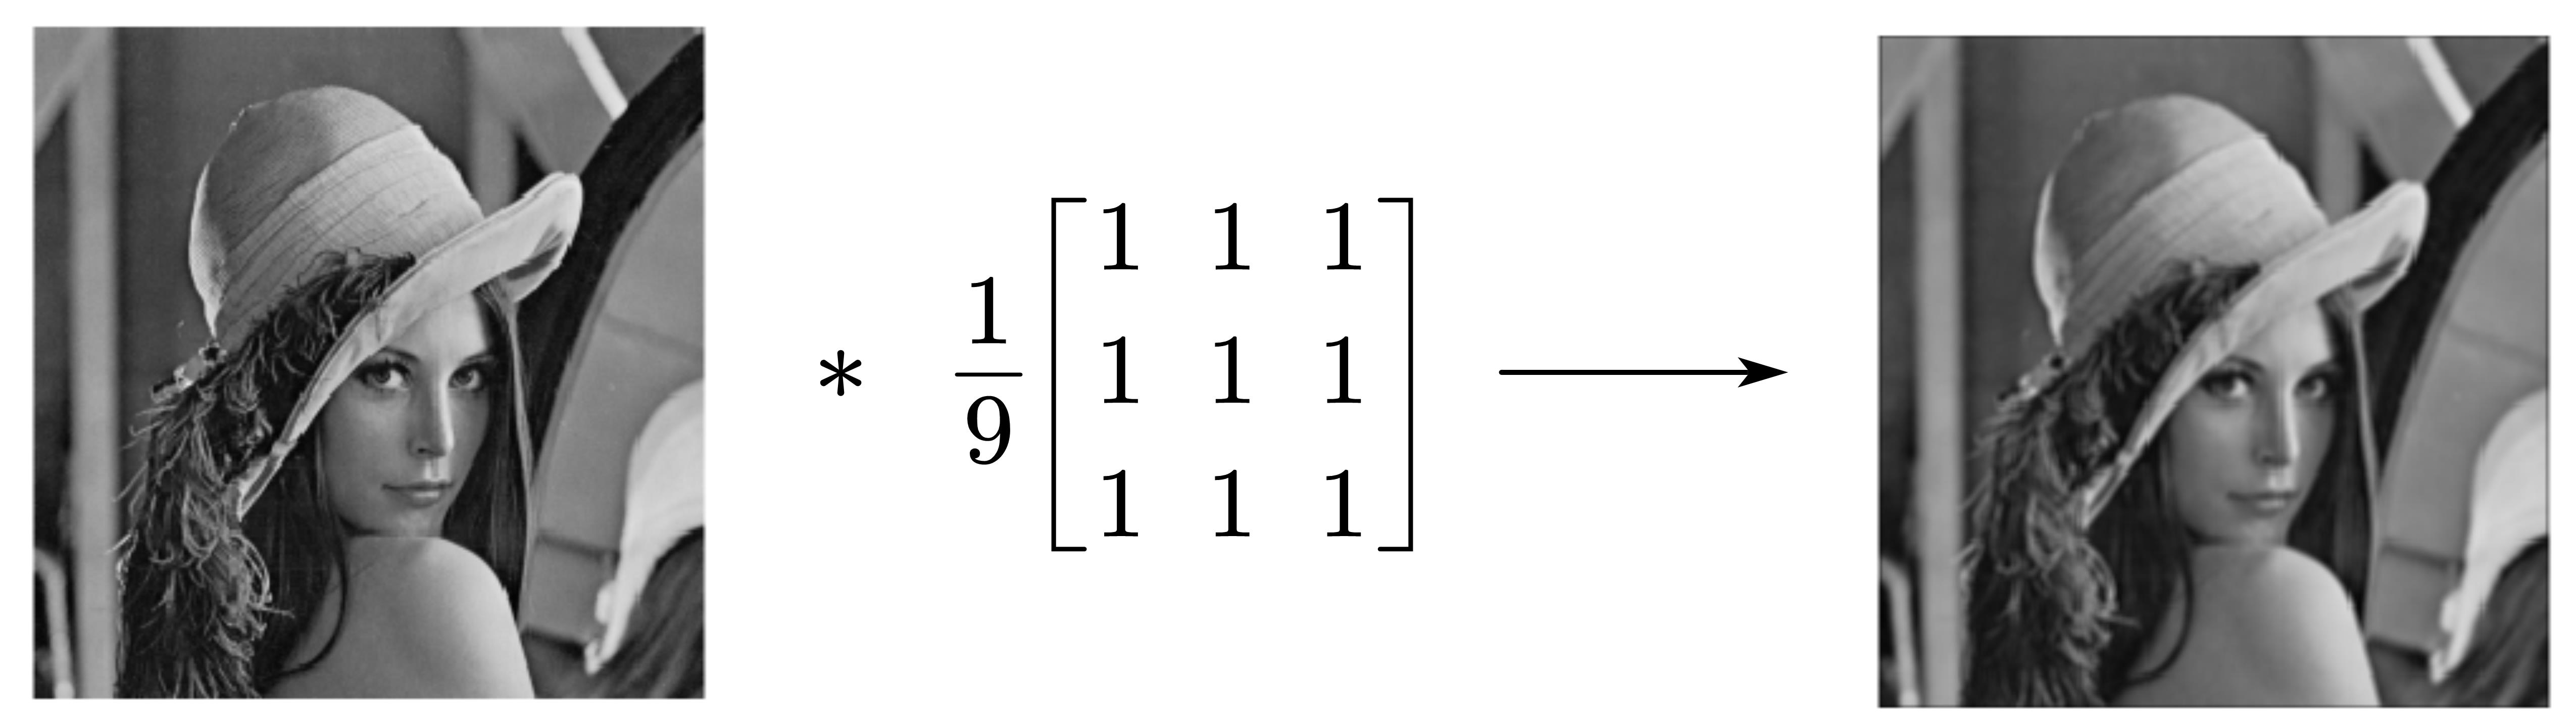
\includegraphics[width=0.8\textwidth]{lena5.jpg}
        \end{figure}
        \item Gauss Smoothing Filter:
        \begin{figure}
            \centering
            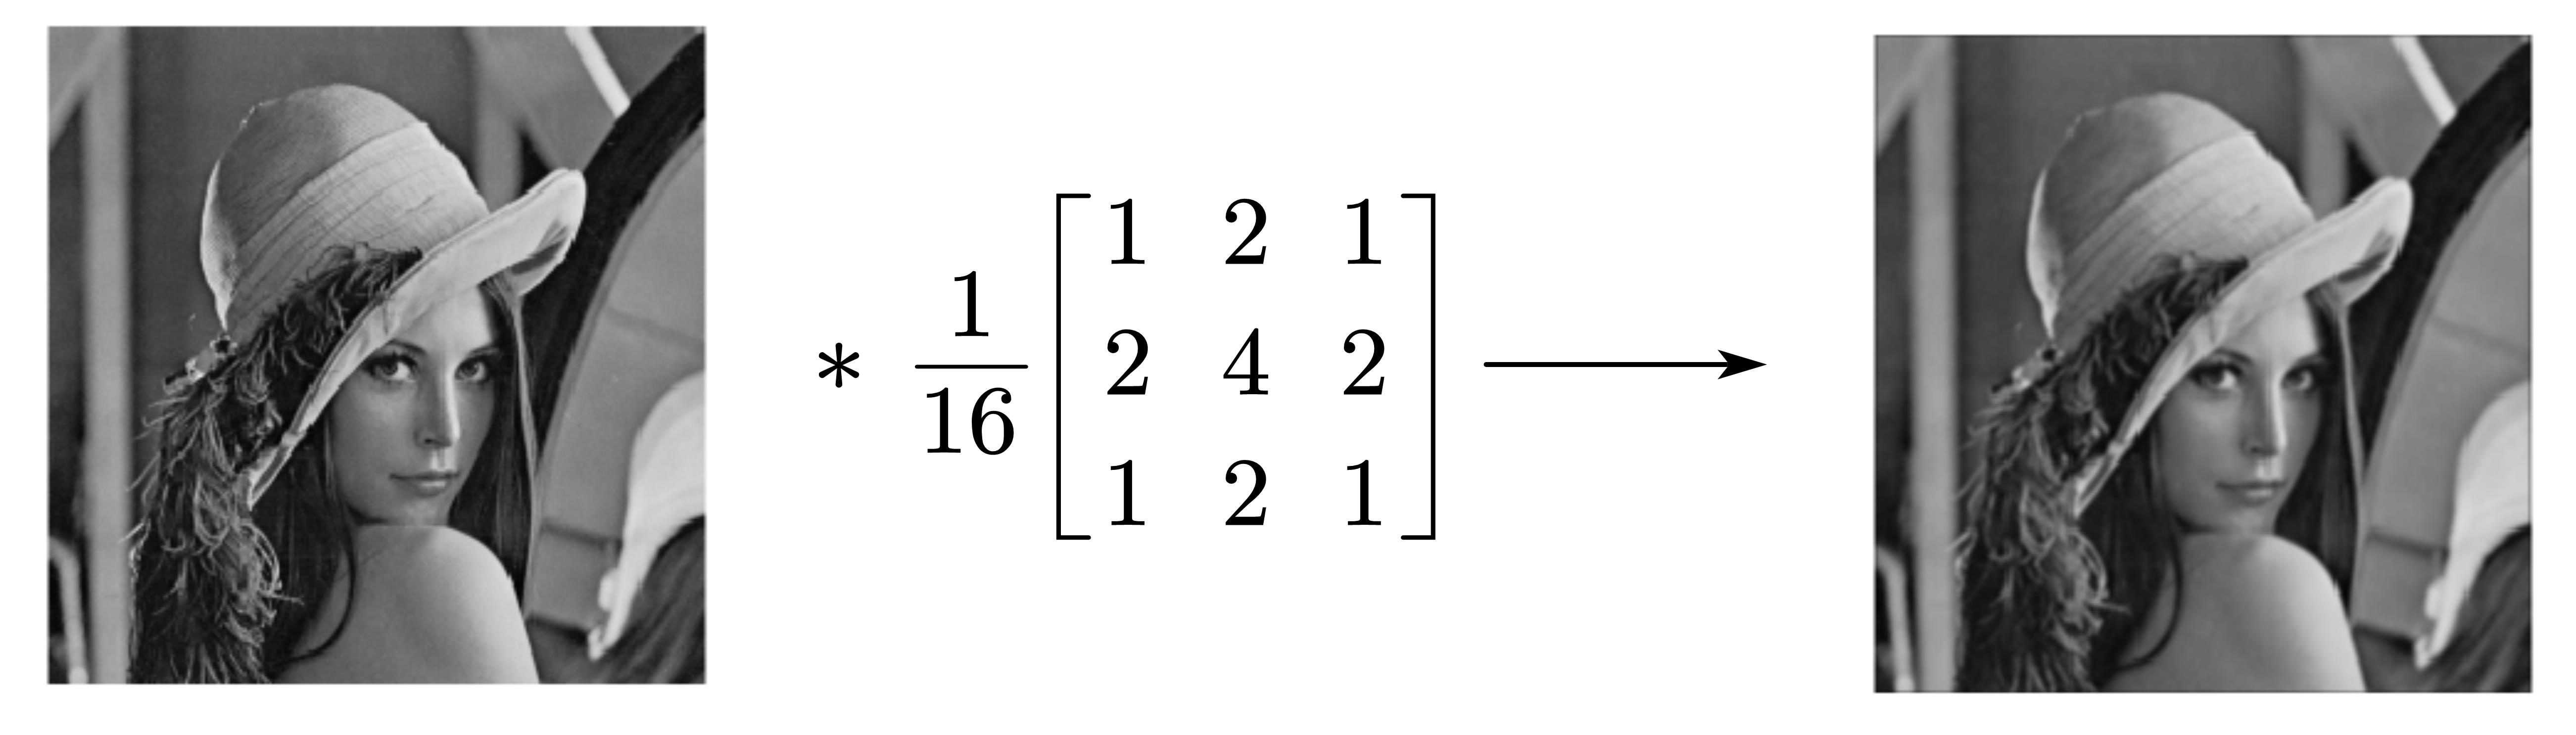
\includegraphics[width=0.8\textwidth]{lena6.jpg}
        \end{figure}
    \end{itemize}
\end{frame}

\begin{frame}{Linear Algebra in Computer Vision}
Gauss Smoothing Filter for many times:
        \begin{figure}
            \centering
            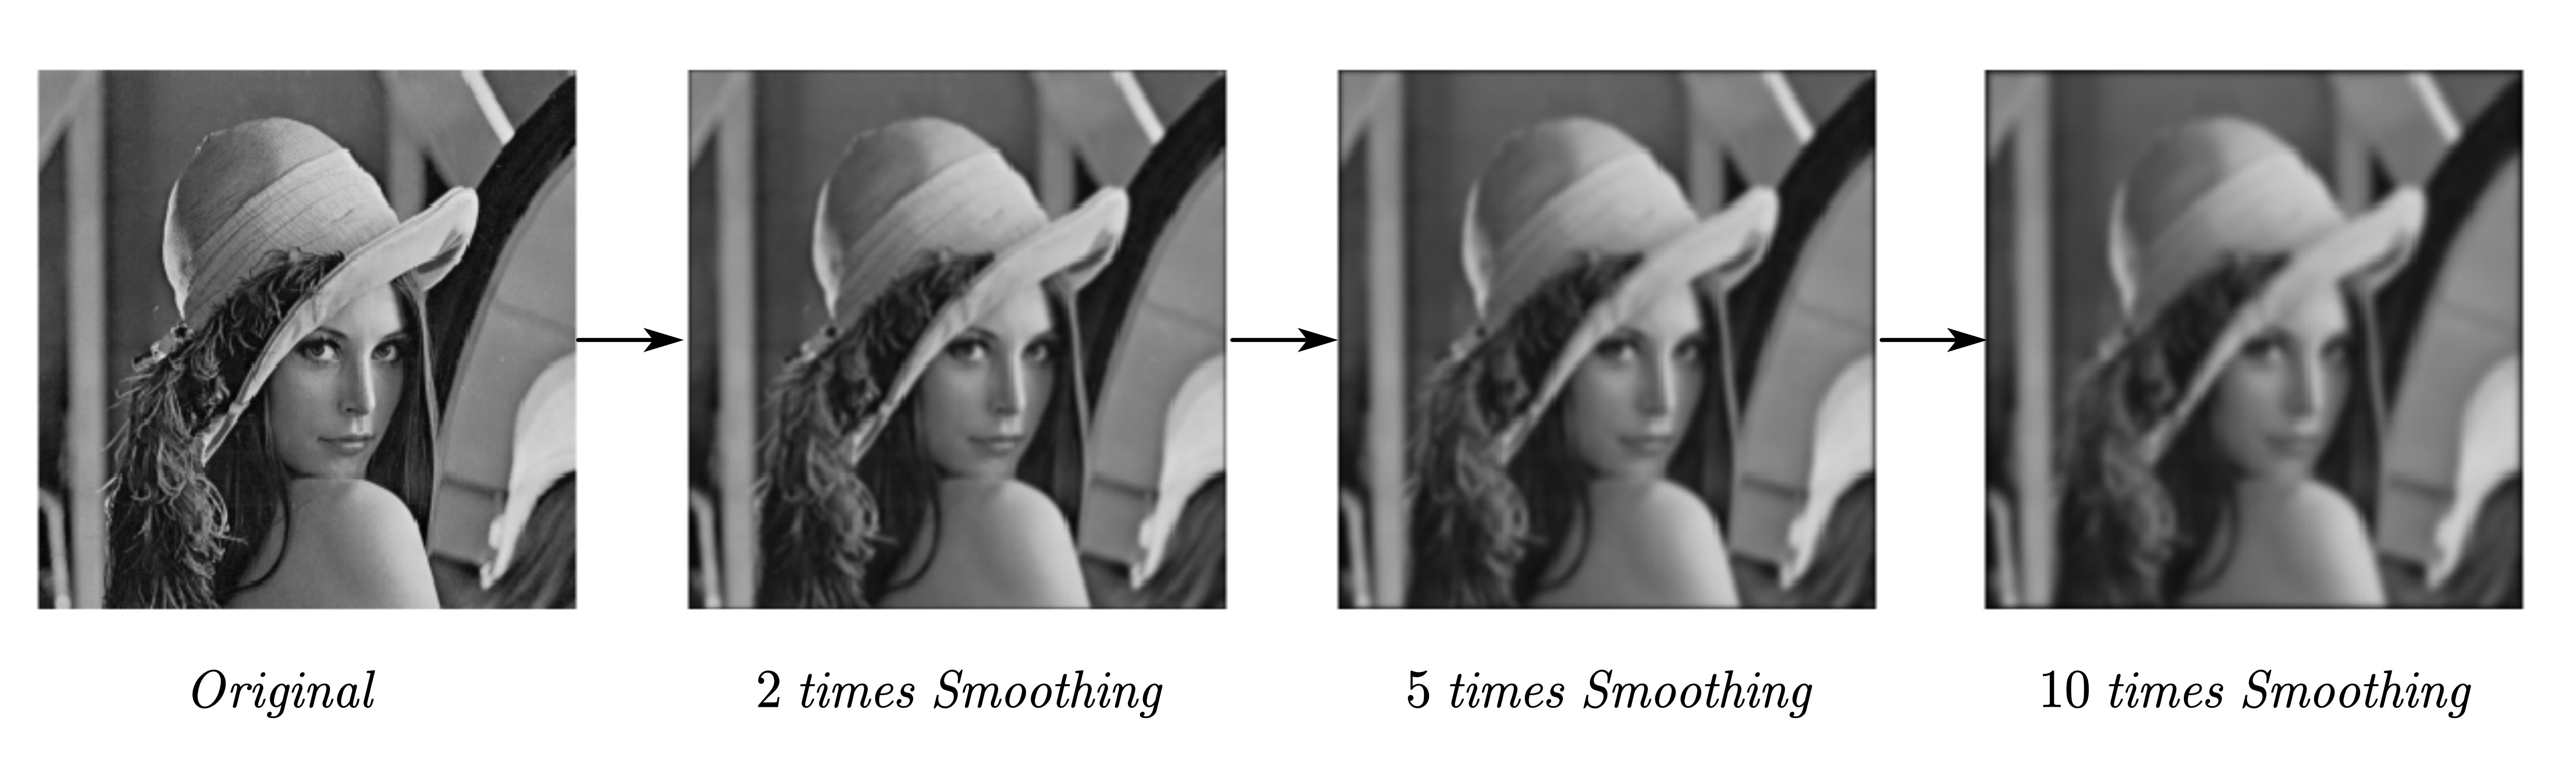
\includegraphics[width=1\textwidth]{lena7.jpg}
        \end{figure}
        Every time when you use the mobile phone, if you try to pull down the notification badge, Gauss Smoothing Filter is applied. That is the magic from Linear Algebra!
\end{frame}

\section{Orthonormal Vectors and Orthogonal Matrices}
\begin{frame}{Orthonormal Vectors}
\begin{definition}
    The vectors $q_1,q_2,\cdots,q_n$ are orthonormal if
    \begin{equation*}
        {q_i}^Tq_j=\begin{cases}
            0, if\,\,i\ne j\\
            1, if\,\,i=j\\
        \end{cases}
    \end{equation*}
\end{definition}

What are the properties of orthonormal vector set?
\begin{itemize}
    \item Any 2 vectors are orthogonal.
    \item Every vector has a length of 1.
\end{itemize}

Well, give me some orthogonal vector set in $\mathbb{R}^2$.

\vspace{3pt}
(You may want to say the standard basis, that's true definitely, can you find some others?)
\end{frame}

\begin{frame}{Orthogonal Matrices}
If you write the orthonormal vectors in the columns of a matrix (kind of familiar?), then it is an orthogonal matrix $Q$.

\vspace{3pt}
$Qx=0$ has only the zero solution! That is because the column vectors are independent (orthogonal is the maximum independent).

\vspace{3pt}
How can I express the property of orthonormal vector set in matrix language (Think about $Q^TQ$)?


\begin{equation*}
    \left[ \begin{matrix}
        -&		-&		{q_1}^T&		-&		-\\
        -&		-&		{q_2}^T&		-&		-\\
        &		&		\vdots&		&		\\
        &		&		\vdots&		&		\\
        -&		-&		{q_m}^T&		-&		-\\
    \end{matrix} \right] _{m\times n}\left[ \begin{matrix}
        |&		|&		&		&		|\\
        |&		|&		&		&		|\\
        q_1&		q_2&		\cdots&		\cdots&		q_m\\
        |&		|&		&		&		|\\
        |&		|&		&		&		|\\
    \end{matrix} \right] _{n\times m}=I _{m\times m}
\end{equation*}

Are $m,n$ need to be equal? That is: are all orthogonal matrix square?

\vspace{3pt}
If your orthogonal matrix is exactly square, $Q^T=Q^{-1}$. (familiar?)
\end{frame}

\begin{frame}{Orthogonal Matrices}
Why we create orthogonal matrix $Q$? How can it be related to the previous knowledge in this chapter?

\vspace{3pt}
We have learnt the matrix representation of projection onto $C(A)$:
\begin{equation*}
    P=A(A^TA)^{-1}A^T
\end{equation*}

If we write down the matrix representation of projection onto $C(Q)$:
\begin{equation*}
    P=Q(Q^TQ)^{-1}Q^T=QQ^T
\end{equation*}

\vspace{3pt}
Recall 2 properties for projection matrices. Check if $QQ^T$ satisties them?

\vspace{3pt}
In Chapter 3.3 least-squares, if we change $A$ to $Q$, what will we get?
\begin{equation*}
    A^TA\hat{x}=A^Tb\Rightarrow \hat{x}=Q^Tb\Rightarrow \hat{x}_i={q_i}^Tb
\end{equation*}

Which shows us the projection of $b$ on the $i$-th basis of $C(Q)$ is just the inner product of $q_i$ and $b$, that is correct because $||q_i||=1$.
\end{frame}

\begin{frame}{Gram-Schmidt}
We have known that orthogonal matrices have those "good" properties, a natural thought is: can I generalize and use the properties for all matrices?

\vspace{3pt}
That is the same to ask: can I transform any linearly independent vector set to orthonormal vector set? Gram and Schmidt answer yes!

\vspace{3pt}
Everything is difficult if you don't choose a easy example to analyze...How about 2 non-orthogonal independent vectors in $\mathbb{R}^2$?
\end{frame}




\end{document}